% !TEX root = ../main.tex

\chapter{RMI on BMv2}
\label{ch:rmionbmv2}

The next chapter of this work is dedicated to the idea of implementing RMI using the reference P4 software switch BMv2. As briefly described in section \ref{sect:background:rmi}, a RMI lookup heavily relies on floating point arithmetic but besides that does not need a lot of other operations to work properly. Therefore a major part of this chapter will be about dealing with these floating point operations. For a simpler start as well as for learning a lot of the basics of the P4 language the BMv2 software switch is used. This does bring quite a lot of advantages to begin with, but as decribed later in section \ref{sect:rmionbmv2:evaluation} does also lead to large differences between what is doable in theory in software and what is actually possible in a real world scenario.

\section{BMv2 and Mininet}
BMv2 stands for behavioral model version two and is the official reference P4 software switch implementation found at \cite{bmv2}. It is written in C++ and can take in and interpret a compiled P4 program and simulate the packet-processing behaviour specified in said P4 program. The implementation runs out of the box on traditional linux distributions and can be combined with virtual network simulation softwares such as \cite{mininet}. Altogether though with regard to this work, neither BMv2 nor Mininet are meant to be production-grade implementations in their area. This means that there are on one side in the case of BMv2 a lot less restrictions imposed than a real world switch would and on the other side for both tools there is a lot less processing speed and throughput potential available than real world equipment would provide.\\

With that out of the way the network architecture simulated by Mininet is extremely simple and barely even worth mentioning. Figure \ref{fig:network_architecture}, in the next section, shows our simple setup and where the BMv2 software switch comes into play together with more detail about the packet flow.

\section{Network setup and packet structure}
\label{sect:rmionbmv2:network}
When looking at how the SOSD benchmark implementation handles many different algorithms at the same time it becomes apparent that separating a phase where an algorithm can do its processing to return a result bound and on the other hand performing the so called last mile search on this remaining bound is key for most learned competitors. This separation comes in handy since performing an efficient search on a given range of data on a P4 switch is not easily doable as of today and therefore this task remains on the host by choice. This leads to the setup shown in figure \ref{fig:network_architecture}. In principle a host sends a regular ethernet packet containing all the usual fields such as destination and source MAC address to the switch. Importantly though the packet sets the ether type field to a custom value of $0x8008$ and appends a payload containing the desired lookup key and space for the response in form of a field for the guessed position and a field for the expected error calculated during the learning phase as visualized in figure  \ref{fig:packet_structure}. As a next step the switch performs the actual RMI calculations, completes the guessed position and expected error field in the packet and forwards the packet back to the source MAC address. The last step that was previously abstracted away is now performed upon receiving the forwarded response packet on the host, meaning that some sort of last mile search is performed in the interval between \([estimated - error, estimated + error]\) to finally find at which position the initially desired lookup key is to be found.\\

In terms of flexibility there is absolutely no restriction of where to forward the finalized RMI packet containing the estimated position and caluclated error to. There are all sorts of possibilites here to use the full power of P4 and network programmability to achieve combinations of packet forwarding and lookup operations. Annother flexibility is the sort of search that is used on the host on the narrowed down search bound. For this work as well as in the SOSD benchmark a regular form of binary search is used, but for different concrete use cases other algorithms may be preferable.

\begin{figure}[ht]
  \centering
  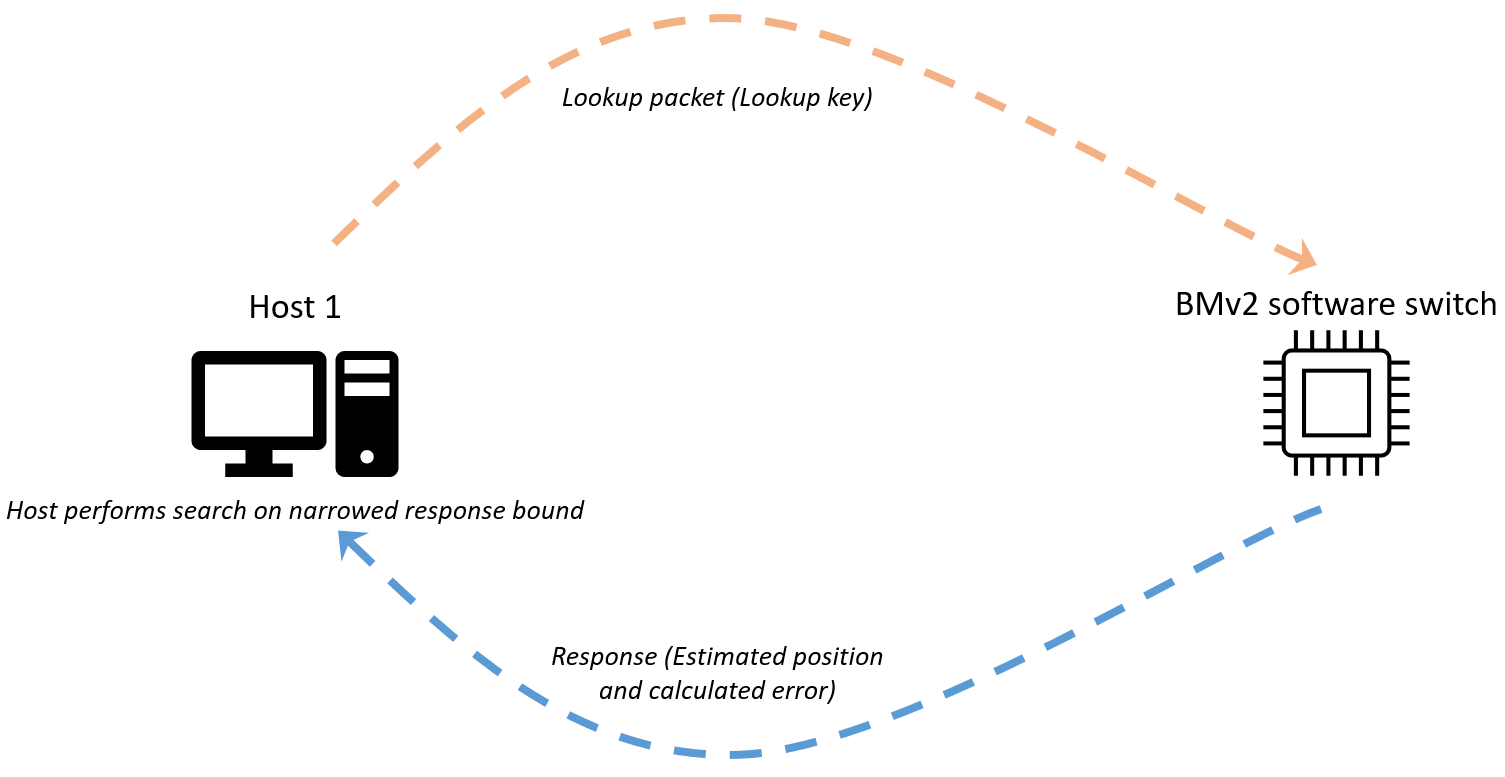
\includegraphics[width=1\textwidth]{network_architecture}
  \caption[Network architecture]{
    \textbf{Mininet network architecture.} Simple network architecture and packet flow proposition to run RMI on a P4 capable switch.
  }
  \label{fig:network_architecture}
\end{figure}

\begin{figure}[ht]
  \centering
  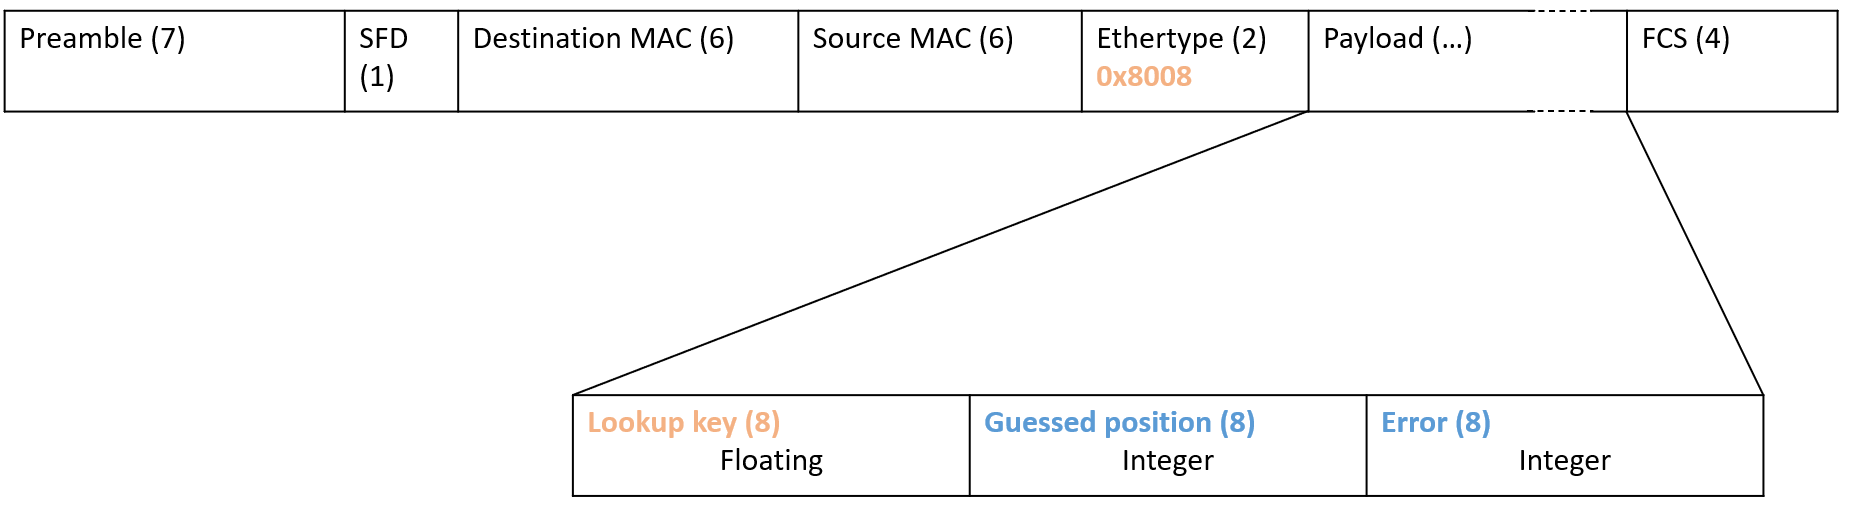
\includegraphics[width=1\textwidth]{packet_structure}
  \caption[RMI packet structure]{
    \textbf{Learned RMI packet structure.} Visualization of an RMI ethernet packet containing the custom ethertype and payload. Field sizes are shown in octets.
  }
  \label{fig:packet_structure}
\end{figure}

\section{Implementation}
\label{sect:rmionbmv2:implmentation}
The reference RMI implementation does generate C++ code depending on the specific dataset it is trained on. This part of the algorithm though is not yet part of this chapter and will be explored more in depth in chapter \ref{ch:rmiforp4}. As a first step to try to translate existing RMI code in C++ into P4 our approach was to decide for a single dataset as well as some constant input parameters. The result of this is that whenever running the existing RMI implementation the exact same C++ code is generated. An example can be found in the appendix in section \ref{sect:appendix:books_200M_uint32_0}. The next step would be to examine the generated code and finally implement the exact same behaviour in P4 by hand. For this multiple challenges must be tackled. One of them being the load function where quite a large chunk of binary layer one parameter data is loaded into memory. Annother one becoming apparent when observing that in this case the learning phase decided for layer zero to use a cubic function and for layer one to use a linear function. The implementations of both of these functions are short as shown in figure \ref{fig:linear_cubic}, but since they solely rely on using the FMA instruction it will turn out that they are going to be quite tricky to translate to P4. In other words a second challenge will be to implement an operation that behaves similarly to the commonly in hardware implemented fused multiply-add CPU instruction in P4.

\captionsetup[figure]{skip=-10pt} % move caption up towards listing
\begin{figure}[ht]
  \begin{C++}
inline double linear(double alpha, double beta, double inp) {
  return std::fma(beta, inp, alpha);
}

inline double cubic(double a, double b, double c, double d, double x) {
  auto v1 = std::fma(a, x, b);
  auto v2 = std::fma(v1, x, c);
  auto v3 = std::fma(v2, x, d);
  return v3;
}\end{C++}
  \caption[Linear and cubic lookup implementation in C++]{ C++ lookup implementation for the linear and cubic model. }
  \label{fig:linear_cubic}
\end{figure}

\subsection{FMA in P4}
\label{sect:rmionbmv2:fma}
This section focusses on a software implementation of the fused multiply-add instruction in P4. The goal is to potentially provide a proof of concept and put performance or optimization considerations aside for now. In section \ref{sect:rmionbmv2:evaluation} a more top down look on things will be given together with some thoughts in form of an evaluation in what way this was a good idea or not.\\

The FMA instruction takes in three parameters and calculates the value resulting from \((x * y) + z\) rounded only once. This means that in order to implement an FMA instruction in P4 one needs to be able to multiply two floating point values as well as adding two floating point values together. This consequently means that there has to be some sort of representation in P4 for a floating point value. This is pretty easily doable by defining a custom header type that follows the official IEEE754 floating point standard published by the \cite{ieee754} shown in figure \ref{fig:double_header}. For 64-bit double values the standard describes a 1-bit field representing the sign, an 11-bit field representing the exponent stored as non-negative biased binary number and finally a 52-bit field representing the mantissa stored as a regular binary number excluding the so called "hidden bit". With this definition set floating point addition as well as floating point multiplication can be addressed.\\

Floating point addition works by first setting the hidden bit on both mantissa fields. Next at its core, by looking at the exponent difference between the two floating point values and shifting the mantissa of the smaller value to the right by that amount. With both mantissas now in the same exponent base, they can be added together with a regular bit addition operation. Lastly both the resulting sign as well as the exponent are determined by the larger floating point value. With this the mathematical addition result is calulcated but the representation is not yet sound, meaning that that due to the calculation the first significant mantissa bit might not be at position 53 where the so called hidden bit is supposed to be. To correct this a normalzation procedure is run where the mantissa and exponent are shifted and adapted such that the first significant mantissa bit moves to position 53 and will finally be omitted to increase the representable value range. In P4 this operation is implemented by ternary matching the calulcated mantissa against a static normalzation table which is shown in a narrowed down form in the appendix in section \ref{sect:appendix:floating_normalization}. The implementation of the addition operation can be found in the appendix in section \ref{sect:appendix:floating_addition}.\\

On the other hand floating point multiplication works similarly by first setting the hidden bit on both mantissa fields. Next, to determine the resulting sign, both input sign bits are XOR-ed together. Further, to determine the resulting exponent, the two unbiased input exponents are added together with a regular bit addition operation. Finally the two mantissa fields are mutliplied together this time with a regular bit multiplication operation and shifted back into their initial exponent space. At this point the mathematical multiplication result is caluclated but again the representation is not yet sound. To correct this the exact same normalzation procedure described in the previous paragraph is run. The implementation of the multiplication operation can be found in the appendix in section \ref{sect:appendix:floating_multiplication}.\\

To finish this section now with both mathematical base operations in place, the final FMA control in P4 does simply execute both of the just described operations one after the other.

\captionsetup[figure]{skip=-10pt} % move caption up towards listing
\begin{figure}[ht]
  \begin{P4}
typedef bit<1> sign_t;
typedef bit<11> exponent_t;
typedef bit<52> mantissa_t;

struct double_t {
  sign_t sign;
  exponent_t exponent;
  mantissa_t mantissa;
}\end{P4}
  \caption[Double header definition in P4]{
    \textbf{IEEE754.} P4 header definition following the IEEE754-2019 standard for 64-bit double values.
  }
  \label{fig:double_header}
\end{figure}

\subsection{Loading model parameters in P4}
With the calculation heavier operations out of the way a next challenge is to have access to the data from the binary file normally directly loaded into memory in C++ representing the so called model parameters that are accessed depending on the resulting calculations of the previous layer. To solve this problem a combination of control plane and data plane is needed. On one side the data plane does predefine an empty table description that later can be filled, while the switch is runnning, from the control plane via the P4Runtime API specified and maintained by \cite{p4runtime-spec}. An example of such a table definition is given in the appendix in section \ref{sect:appendix:rmi_table}. The data plane on the other side now simply reads the existing model parameters file and sends these informations over to the switch. This is done with Python since the P4Runtime environement is implemented in Python. To work correctly the script takes in the location of the binary model parameters file as well as the necessary connection parameters to establish a connection to the switch. The table entries are sent in batches to the switch for acceptable performance in the simulated network environement but besides that the implementation is trivial. On the data plane side of things again, whenever a lookup packet arrives and a layer needs access to model parameters the P4 program performs an exact table match with the reulting index from the previous layer to determine the parameters for the next layer.

\subsection{The actual lookup function}
Finally with the described functions implemented the actual lookup control simply becomes a matter of putting it all together as shown in the appendix in section \ref{sect:appendix:rmi_lookup}. One additional but relatively simple function that had to be implemented was a function that casts a floating point value to an integer in P4. As a basic concept each layer takes in its layer parameters as arguments and returns a prediction index for the next layer. In the example case of the books\_200M dataset with 32-bit keys a two-layer RMI is generated where the first layer follows a cubic model and takes in the statically in the C++ header file (shown in \ref{sect:appendix:books_200M_uint32_0}) present L0 parameters. After doing the FMA calculations for said cubic layer, the result is cast back to an integer which is then used as an index to perform an exact table match with the table described in the previous section to retrieve the L1 parameters used as input for the linear model. Finally the FMA calulations for the linear model are computed and after casting the floating point result back to an integer value, the guessed index is clamped to a value between zero and the dataset size and finally returned.

\section{Evaluation}
\label{sect:rmionbmv2:evaluation}
When running and testing the described setup including the virtual network and the software emulated network switch, the possibilites are obviously very limited. Still though, when looking at accuracy when sending one million test lookups generated by the SOSD benchmark, the P4 implementation on the switch achieves a 100\% prediction accuracy. Meaning for all lookup packets sent, the precomputed lookup key is actually to be found in the range given by the guess and the error returned in the response packet.\\

In any case accuracy is fine and for the scope of this work rather pleasing but the implementation as is does ignore quite a lot of real world limitations. A first one of them being for example that currently available switches do mostly not support multiplication on their ALUs. This does break the floating point multiplication function, which is needed for the FMA implementation which in turn is needed for different model lookup implemenations. Annother one of these limitations being that current real world switches are limited to a certain amount of ALU stages. Meaning that for the switch to reach optimal operation speed, a packet can maximally perform a certain amount of computation. For now since not having any ALU hardware support for floating point arithmetic all mathematical operations are implemented in software and therefore in the current implementation this limit of ALU stages is more than exceeded. A next limitation is discussed in the following section where current switches are very limited in terms of what bit width ALUs can handle for basic operations. A final limitation or moreso a very large negative point comes from the fact that the FMA operation is fully implemented in software. This not only leads to the previously described overfull stage usage but also to bad performace in comparision to hardware implemented FMA instructions on a server's CPU where not only the hardware itself means a significant speed up but also the fact that FMA circuits can often benefit from smarter design choices instead of just performing one mathematical operation after the other.\\

All in all with so much of these limitations on the table, the goal and purpose of this work and of this implemenation definetely and at best becomes a theoretical proof of concept, showing what could potentially be possible. While reaching expected prediction accuracy a lot of progress in terms of extending ALU capability on real world switches needs to be done in order to enable RMI the way it was proposed in this chapter.

\subsection{32-bit width attempt}
As already mentioned currently existing real world switches often have ALUs that can maximally treat and compute values up to 32-bit width. With this in mind the first attempt made for all the steps described in this chapter was also limited to floating point values following the IEEE754 single floating point standard. While initially working quite well and being a bit simpler to deal with in terms of readability, when testing lookup accuracy it pretty quickly became clear that the amount of accuracy that single floating point values offer was simply not precise enough for RMI to work properly. This especially holds true due to the fact that all the generated model parameters are designed to use double floating point values. Changing the inner workings of the RMI learning phase to use larger error bounds or cope with the smaller accuracy in annother way would have very quickly overshot the scope of this work, especially when looking at how much complexity and work was already put into this part of the algorithm by other people.
